%!TEX program = xelatex
\documentclass[12pt,a4paper,oneside]{book}

% ==========================================
% BASIC PACKAGES
% ==========================================
\usepackage[utf8]{inputenc} % for UTF-8 encoding
\usepackage{tabularx}
\usepackage{array}
\usepackage{fontspec} % for font selection
\setmainfont{Times New Roman} % set main font to Times New Roman
\usepackage[a4paper, left=4cm, right=3cm, top=3cm, bottom=3cm]{geometry} % set page margins
\usepackage[bahasa]{babel} % untuk bahasa Indonesia
\usepackage{csquotes} % for context-sensitive quotation facilities
\usepackage{setspace} % for line spacing
\onehalfspacing % spasi 1.5
\usepackage{graphicx} % for images
\usepackage{caption} % for customizing captions
\usepackage{subcaption} % for sub-figures
\usepackage{hyperref} % for hyperlinks
\usepackage{titlesec} % for customizing titles
\usepackage{tocloft} % for customizing table of contents
\usepackage{lipsum} % for dummy text (lorem ipsum text)
\usepackage{floatrow} % for customizing float (figure and table) positions
\usepackage{listings} % for code listing
\usepackage{amsmath} % for math
\usepackage{float}
\usepackage{amssymb} % for math symbols
\usepackage[shortlabels]{enumitem} % for customizing lists
\setlist[enumerate]{nosep, topsep=-10pt} % mengurangi spasi antar item dan atas bawah daftar
\setlist[itemize]{nosep, topsep=-10pt} % mengurangi spasi antar item dan atas bawah daftar
\usepackage[skip=12pt]{parskip}
\usepackage{longtable}
\usepackage{booktabs}
\usepackage[id-ID]{datetime2}
\usepackage{enumitem}

\setcounter{tocdepth}{4} % kedalaman daftar isi sampai subsubbab
\setcounter{secnumdepth}{4} % kedalaman penomoran sampai subsubbab

% ==========================================
% SITASI DAN DAFTAR PUSTAKA (MENGGUNAKAN CHICAGO MANUAL OF STYLE)
% ==========================================
\usepackage[
    backend=biber,
    authordate,
    language=english,
    autolang=other
]{biblatex-chicago}

\addbibresource{daftar-pustaka.bib}

% ==========================================
% Ubah istilah bahasa Inggris di daftar pustaka ke Bahasa Indonesia
% ==========================================
\DefineBibliographyStrings{english}{
  and          = {dan},
  andothers    = {dkk.},
  editor       = {penyunting},
  editors      = {penyunting},
  translator   = {penerjemah},
  byeditor     = {disunting oleh},
  bytranslator = {diterjemahkan oleh},
  in           = {dalam},
  edition      = {edisi},
  pages        = {hal.},
  page         = {hal.},
  volume       = {vol.},
  number       = {no.},
  urlseen      = {diakses pada},
  url          = {tautan},
}

% ==========================================
% Pastikan \cite() menampilkan (Penulis Tahun)
% ==========================================
\let\oldcite\cite
\renewcommand{\cite}{\parencite}

% ==========================================
% Atur pemisah nama penulis agar lebih natural dalam Bahasa Indonesia
% ==========================================
\renewcommand*{\finalandcomma}{} % hilangkan koma sebelum 'dan'


% ==========================================
% TAMPILAN
% ==========================================
\hypersetup{
    colorlinks=true,
    linkcolor=black,
    citecolor=black,
    urlcolor=black
}

% -- No Header dan No Footer ---
\pagestyle{plain}

% --- Ubah nama daftar listing ke "DAFTAR ALGORITMA" ---
% --- Harus diletakkan sebelum \begin{document} ---
\renewcommand{\lstlistlistingname}{\centering\normalsize DAFTAR KODE} 
\renewcommand{\lstlistingname}{Kode}
\lstset{basicstyle=\ttfamily\footnotesize,breaklines=true}

\renewcommand \cftchapdotsep{4.5}

% ==========================================
% AWAL DOKUMEN
% ==========================================
\begin{document}

% ==========================================
% HALAMAN JUDUL
% ==========================================
\begin{titlepage}
\begin{center}

    \vspace*{2cm}
    
    {\Large\bfseries Pengembangan Sistem Prediksi Risiko Hipertensi Menggunakan Machine Learning Terinterpretasi (SHAP) dan Chatbot Berbasis LLM-RAG}\\
     \vspace{4cm}

    {\Large \textbf{Proposal Tugas Akhir}}\\

    \vspace{2cm}
    
    {\large Oleh}\\[0.3cm]
    \textbf{
    {\large Samuel Franciscus Togar Hasurungan}\\
    {\large 18222131}
    }\\

    \vspace{2cm}
    
    \begin{figure}[h]
    \centering
    \includegraphics[width=0.2\textwidth]{image/ganesha.jpg}
    \end{figure}
    
    \vfill

    \textbf{
    {\large PROGRAM STUDI SISTEM DAN TEKNOLOGI INFORMASI}\\
    {\large SEKOLAH TEKNIK ELEKTRO DAN INFORMATIKA}\\
    {\large INSTITUT TEKNOLOGI BANDUNG}\\
    {\large \DTMlangsetup{showdayofmonth=false,showmonthname=true,showyear=true}\today}
    }
\end{center}
\end{titlepage}

% ==========================================
% LEMBAR PENGESAHAN 
% ==========================================
\newpage
\thispagestyle{empty}
\pagenumbering{gobble}
\begin{center}
  \textbf{\large LEMBAR PENGESAHAN}\\[1cm]
  \vspace*{1.5cm}
    
  % JUDUL DISAMAKAN DENGAN HALAMAN JUDUL
  {\large\bfseries Pengembangan Sistem Prediksi Risiko Hipertensi Menggunakan Machine Learning Terinterpretasi (SHAP) dan Chatbot Berbasis LLM-RAG}\\
     \vspace{2cm}

  {\Large \textbf{Proposal Tugas Akhir}}\\

  \vspace{1.5cm}
  
  {\large Oleh}\\[0.3cm]
    \textbf{
    {\large Samuel Franciscus Togar Hasurungan}\\
    {\large 18222131}
  }\\
    
  \vspace{0.5cm}
 
  {\large Program Studi Sistem dan Teknologi Informasi}\\
  {\large Sekolah Teknik Elektro dan Informatika}\\
  {\large Institut Teknologi Bandung}\\

  \vspace{1.5cm}

  Proposal Tugas Akhir ini telah disetujui dan disahkan\\ 
  di Bandung, pada tanggal \today\\[1cm]

% ==========================================
% Versi 1 pembimbing (default)
% ==========================================
	Pembimbing  \\[3cm]
	Prof. Dr. Ir. Suhono Harso Supangkat, M.Eng.   \\[0.2cm]
	NIP. 196212031988111001 
\end{center}

\vspace{1cm}
\noindent

% ==========================================
% Jika ada 2 pembimbing TA, sesuaikan bagian di bawah
% ==========================================
%\begin{tabular}{p{1cm}p{7cm}p{7cm}}
%   & Pembimbing 1 & Pembimbing 2 \\[3cm]
%   & Prof. Dr. Ir. Suhono Harso Supangkat, M.Eng. & Dr. Mary Doe, M.Sc. \\[0.2cm]
%   & NIP. 196212031988111001 & NIP. 987654321
%\end{tabular}

% -- Change page number style to roman ---
\pagenumbering{roman} 

% ==========================================
% DAFTAR ISI, TABEL, GAMBAR
% ==========================================
% --- DAFTAR ISI ---
\makeatletter
\renewcommand{\tableofcontents}{%
  \clearpage
  \thispagestyle{plain}% no header
  \begin{center}
    {\large\bfseries\MakeUppercase{\contentsname}\par}
  \end{center}
  \vskip 1em
  \@starttoc{toc}%
}
\makeatother

\newpage
\renewcommand{\cfttoctitlefont}{\hfill\large\bfseries\MakeUppercase}
\renewcommand{\cftaftertoctitle}{\hfill}
\tableofcontents

% --- DAFTAR GAMBAR ---
\newpage
\renewcommand{\cftloftitlefont}{\hfill\large\bfseries\MakeUppercase}
\renewcommand{\cftafterloftitle}{\hfill}
\listoffigures
\addcontentsline{toc}{chapter}{DAFTAR GAMBAR}

% --- DAFTAR TABEL ---
\newpage
\renewcommand{\cftlottitlefont}{\hfill\large\bfseries\MakeUppercase}
\renewcommand{\cftafterlottitle}{\hfill}
\listoftables
\addcontentsline{toc}{chapter}{DAFTAR TABEL}

% --- DAFTAR LISTING (ALGORITMA, PSEUDOCODE, SOURCE CODE) ---
\newpage
\lstlistoflistings
\addcontentsline{toc}{chapter}{\lstlistlistingname}

\mainmatter
% --- FORMAT TAMPILAN JUDUL BAB, SUBBAB, JUDUL GAMBAR DAN TABEL ---
% --- Judul Bab ---
\titleformat{\chapter}[display]
      {\centering\normalfont\large\bfseries} % Commands for the entire chapter title
      {\MakeUppercase \chaptertitlename\ \thechapter}{0pt}{\large} % Chapter number format
\renewcommand\thechapter{\Roman{chapter}}
% --- Judul Subbab dan Subsubbab ---
\titleformat{\section}
	{\normalfont\bfseries}
	{\thesection}{1em}{}
\titleformat{\subsection}
	{\normalfont\bfseries}
	{\thesubsection}{1em}{}
\titleformat{\subsubsection}
	{\normalfont\bfseries}
	{\thesubsubsection}{1em}{}


% --- Format judul gambar dan tabel ---
\captionsetup[figure]{labelsep=space}
\captionsetup[table]{labelsep=space}
\floatsetup[table]{capposition=top}
\captionsetup[lstlisting]{labelsep=space}
\floatsetup[lstlisting]{capposition=top}

% --- Atur indentasi paragraf ---
\setlength{\parindent}{0pt}
% -- Change page number style to arabic ---
\pagenumbering{arabic} 

% --- INPUT FILES ---
% Pastikan file-file ini ada di folder yang sama
\input{Bab I - Pendahuluan.tex}
\input{Bab II - Studi-Literatur.tex}
% % ============================================================================================
% BAB III ANALISIS MASALAH
% VERSI PERBAIKAN (04-Nov-2025)
% FIX:
% 1. Mengganti float '[t]' (top) menjadi '[H]' (Here) dari paket 'float'.
%    Ini "memaksa" tabel untuk tampil persis di tempat kode diletakkan
%    dan tidak mengambang ke bawah halaman.
%
% PENTING: Pastikan Anda sudah menambahkan \usepackage{float} di file .tex utama!
% ============================================================================================
\chapter{ANALISIS MASALAH}
\label{chap:analisis-masalah}

\section{Analisis Kondisi Saat Ini}
\label{sec:analisis-kondisi-saat-ini}

% --- Gambar Alur Proses As-Is ---
% FIX: Menggunakan [H] agar gambar tidak mengambang
\begin{figure}[H] 
	\centering
  \captionsetup{justification=centering}
    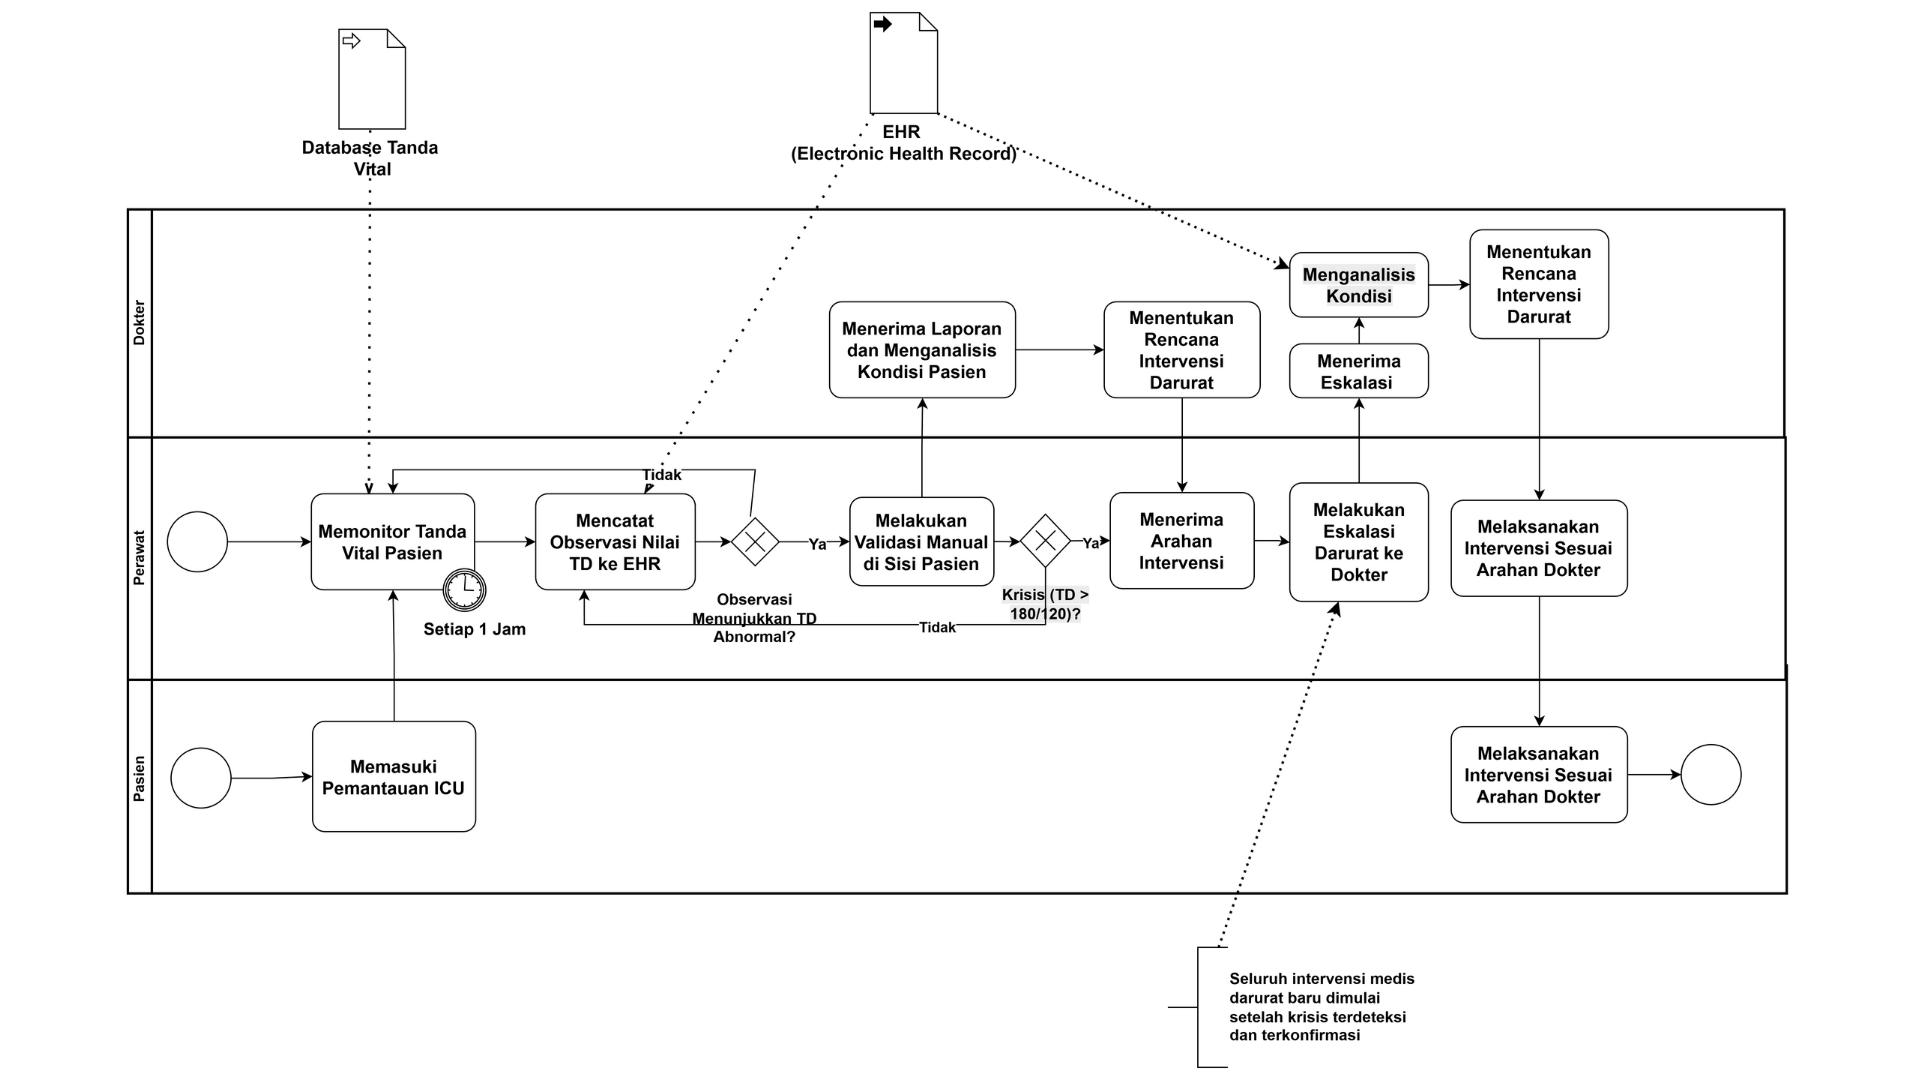
\includegraphics[width=0.9\textwidth]{image/gambar1.png} 
	\caption{Alur proses 'As-Is' manajemen klinis hipertensi}
	\label{gambar:alur-as-is}
\end{figure}

Proses manajemen klinis untuk pasien hipertensi saat ini beroperasi pada paradigma yang fundamentalnya bersifat reaktif. Alur kerja konvensional ini, seperti yang telah dimodelkan, bergantung pada intervensi yang baru dilakukan setelah diagnosis ditegakkan atau setelah terjadi fluktuasi tekanan darah (TD) yang signifikan. Kelemahan utama dari pendekatan ini adalah kegagalannya dalam mengantisipasi dan mencegah episode akut yang paling berbahaya, yaitu krisis hipertensi. Krisis hipertensi didefinisikan sebagai kondisi darurat medis di mana tekanan darah melonjak melebihi 180/120 mmHg. Kondisi ini secara langsung berpotensi menyebabkan kerusakan pada organ target, seperti stroke atau gagal jantung, sehingga menjadikannya tantangan serius bagi kesehatan masyarakat. Dengan demikian, alur kerja yang hanya menunggu terjadinya krisis adalah model yang secara inheren berisiko tinggi dan tidak memadai.

Urgensi untuk mengatasi masalah ini diperkuat oleh definisi klinis dari krisis hipertensi itu sendiri. Kondisi ini diklasifikasikan sebagai Hypertensive Emergency (Hipertensi Emergensi) ketika lonjakan TD yang parah (melebihi 180/120 mmHg) disertai dengan bukti adanya kerusakan organ target akut. Kerusakan ini dapat bermanifestasi secara cepat dan parah, meliputi perubahan status mental, infark miokard, gagal ginjal akut, atau diseksi aorta. Dalam paradigma "As-Is", alarm atau eskalasi ke dokter baru terjadi setelah kondisi yang mengancam jiwa ini dimulai, sehingga waktu penanganan yang krusial telah hilang. Identifikasi dan tatalaksana yang segera sangat penting untuk mencegah kerusakan organ permanen atau risiko kematian. Oleh karena itu, jelas bahwa sistem yang hanya "bereaksi" terhadap krisis yang sudah terjadi secara fundamental gagal dalam misi preventif.

Kebutuhan untuk bertransisi menuju manajemen proaktif kini menjadi mungkin berkat kemajuan dalam pengumpulan data dan machine learning. Ketersediaan dataset publik beresolusi tinggi, seperti MIMIC-IV, menyediakan rekaman data longitudinal yang rinci, termasuk data runtun waktu (time-series) dari tanda-tanda vital seperti nilai TD per jam. Data historis yang kaya ini merupakan prasyarat mutlak yang memungkinkan pelatihan model prediktif untuk memantau fluktuasi tekanan darah dari jam ke jam. Dengan memanfaatkan data ini, sebuah sistem dapat dikembangkan untuk memberikan peringatan dini. Tujuan utamanya adalah untuk memprediksi probabilitas terjadinya krisis hipertensi sebelum ambang batas 180/120 mmHg terlampaui, sehingga memungkinkan intervensi preventif.

Meskipun model machine learning (ML) seperti ensemble (Random Forest atau XGBoost) telah menunjukkan kinerja state-of-the-art dalam menangani data tabular kompleks, akurasi prediktif yang tinggi (high-fidelity) saja belum mencukupi untuk adopsi klinis. Hambatan utama dalam implementasi machine learning di lingkungan berisiko tinggi seperti perawatan kesehatan adalah sifat alaminya sebagai "kotak hitam" (black box). Masalah "black box" ini merujuk pada kurangnya transparansi dan interpretabilitas dari model-model kompleks. Meskipun model tersebut mampu menghasilkan prediksi (keluaran) yang sangat akurat, model tersebut tidak dapat memberikan justifikasi yang mudah dipahami manusia atas keputusan yang diambil. Opasitas ini menjadi masalah kritis di bidang kedokteran, di mana setiap rekomendasi otomatis harus dapat diverifikasi dan dipertanggungjawabkan.

Konsekuensi langsung dari masalah "black box" adalah terhambatnya kepercayaan dan akuntabilitas dari pengguna akhir, yaitu para klinisi. Seorang dokter tidak dapat memercayai atau menindaklanjuti sebuah peringatan "Risiko Krisis 85\%" jika sistem tidak dapat memberikan justifikasi yang masuk akal dan dapat ditindaklanjuti secara klinis. Kurangnya transparansi internal ini menciptakan keraguan, karena pengguna tidak dapat memverifikasi alasan di balik peringatan tersebut. Dalam domain di mana keputusan dapat berarti antara hidup dan mati, sistem yang tidak dapat dipertanggungjawabkan tidak akan pernah diadopsi sepenuhnya, tidak peduli seberapa akurat prediksinya. Kesenjangan kepercayaan ini adalah penghalang adopsi yang sama seriusnya dengan masalah paradigma reaktif itu sendiri.

Untuk menjembatani kesenjangan antara akurasi prediktif dan adopsi klinis, disiplin AI yang dapat dijelaskan (Explainable AI atau XAI) menjadi komponen yang krusial dan wajib ada. XAI menawarkan solusi untuk "membuka" kotak hitam dan memberikan transparansi yang dibutuhkan. Metode atribusi post-hoc yang kuat seperti SHAP (SHapley Additive exPlanations) secara khusus dirancang untuk mengatasi masalah ini. SHAP, yang didasarkan pada teori permainan kooperatif, mampu mengkalkulasi kontribusi spesifik dari setiap fitur (misalnya, 'usia', 'TD 3 jam terakhir') terhadap deviasi prediksi model dari nilai dasarnya. Metode ini secara efektif memberikan penjelasan yang terukur (baik secara global maupun lokal per individu) mengenai alasan di balik terbentuknya suatu prediksi risiko. Kemampuan untuk menyediakan rasionalisasi inilah yang akan mengubah model ML dari sekadar alat prediksi menjadi sistem pendukung keputusan yang dapat dipercaya.

% --- Subseksi Analisis Kesenjangan ditambahkan berdasarkan PDF baru ---
\subsection{Analisis Kesenjangan}
Dilakukan analisis kesenjangan berikut ini untuk memetakan secara terstruktur kondisi saat ini (As-Is) dengan kondisi ideal (To-Be) yang diharapkan dari solusi yang diusulkan. Pemetaan ini merangkum permasalahan inti yang dijabarkan dalam Tabel \ref{tbl:gap-analysis} ini.

% --- Tabel Analisis Kesenjangan ---
% FIX: Menggunakan [H] agar tabel tidak mengambang
\begin{table}[H] 
  \begin{tabularx}{\textwidth}{ | l | X | X | X |}
	\hline
	\textbf{Domain Masalah} & \textbf{Kondisi Saat ini (As-Is)} & \textbf{Kesenjangan (Gap)} & \textbf{Kondisi Ideal (To-Be)} \\
	\hline
	Manajemen Klinis (Proses) & 
    Paradigma intervensi bersifat reaktif. Tindakan medis darurat baru diambil setelah pasien mengalami krisis hipertensi (TD $> 180/120$ mmHg). & 
    Keterlambatan intervensi kritis dan risiko kerusakan organ target (stroke, gagal jantung) yang tidak terantisipasi karena kegagalan mendeteksi risiko lebih awal. & 
    Paradigma manajemen bersifat proaktif. Klinisi mendapatkan peringatan dini yang akurat untuk mengantisipasi risiko krisis sebelum terjadi. \\
	\hline
	Adopsi Teknologi & 
    Model machine learning (ML) yang akurat bersifat "black box". Klinisi tidak dapat memahami atau memverifikasi alasan di balik sebuah peringatan risiko. & 
    Hambatan adopsi dan kurangnya kepercayaan (trust) pada sistem cerdas. Sistem tidak akuntabel sehingga sulit diimplementasikan di lingkungan berisiko tinggi. & 
    Model ML bersifat transparan dan dapat dijelaskan. Sistem mampu memberikan justifikasi (via SHAP) untuk setiap prediksi risiko individu, sehingga membangun kepercayaan klinis. \\
	\hline
	Pemanfaatan Data (Sistem) & 
    Data runtun waktu (time-series) klinis beresolusi tinggi (dari MIMIC-IV) ada, namun belum dimanfaatkan secara optimal untuk prediksi antisipatif. & 
    Peluang yang terlewatkan. Data historis yang kaya hanya digunakan untuk analisis retrospektif, bukan untuk memprediksi dan mencegah outcome buruk secara proaktif. & 
    Data time-series diproses melalui alur kerja (pipeline) rekayasa fitur untuk melatih model ML yang mampu mengubah data historis menjadi peringatan dini yang dapat ditindaklanjuti. \\
	\hline
  \end{tabularx}
  \caption{Analisis Kesenjangan (Gap Analysis)}
  \label{tbl:gap-analysis}
\end{table}

Di sini diketahui bahwa masalah yang dihadapi bersifat multifaset, mencakup aspek proses klinis (paradigma reaktif) dan aspek teknologi (masalah "black box"). Kesenjangan ini menunjukkan kebutuhan mendesak akan sebuah solusi cerdas yang tidak hanya menyajikan prediksi outcome, tetapi juga mampu menyajikan rasionalisasi dari prediksi tersebut untuk membangun kepercayaan. Untuk dapat merancang solusi yang efektif dalam menutup kesenjangan ini, langkah selanjutnya adalah menerjemahkan kebutuhan tersebut ke dalam spesifikasi fungsional dan non-fungsional yang terukur.

\section{Analisis Kebutuhan}
Berdasarkan analisis kesenjangan yang telah dipaparkan sebelumnya, langkah selanjutnya adalah menerjemahkan kebutuhan solusi menjadi serangkaian spesifikasi yang terukur. Tahap ini krusial untuk memastikan bahwa sistem yang akan dikembangkan, yaitu purwarupa "Digital Twin Sederhana", secara langsung menjawab dua masalah fundamental yang telah diidentifikasi. Spesifikasi ini akan dibagi menjadi tiga kategori utama: identifikasi masalah spesifik dari kacamata pengguna, kebutuhan fungsional (apa yang harus dilakukan sistem), dan kebutuhan non-fungsional (kriteria kualitas sistem). Proses pendefinisian kebutuhan ini akan menjadi cetak biru (blueprint) yang memandu seluruh alur kerja penelitian, mulai dari akuisisi data hingga perancangan prototipe.

\subsection{Identifikasi Masalah Pengguna}
Pengguna utama dari sistem "To-Be" yang diusulkan adalah Klinisi di lingkungan perawatan intensif, yang mencakup Dokter (sebagai pengambil keputusan) dan Perawat (sebagai pelaksana monitor dan intervensi). Berdasarkan analisis kondisi "As-Is" (3.1), kedua pengguna ini menghadapi dua masalah spesifik yang saling terkait. Masalah pertama adalah beban kognitif dan risiko keterlambatan intervensi akibat paradigma reaktif. Perawat ICU dihadapkan pada beban kerja pemantauan manual yang tinggi, di mana mereka harus mengamati tanda vital pasien secara periodik (misal, per jam). Masalahnya, krisis hipertensi dapat berkembang cepat di antara interval pengecekan, sehingga memunculkan risiko kesalahan manusiawi (human error) atau deteksi yang terlambat. Bagi Dokter, masalahnya adalah mereka baru menerima eskalasi darurat setelah pasien berada dalam kondisi krisis, sehingga kehilangan waktu emas untuk melakukan pencegahan.

Masalah kedua adalah ketidakpercayaan dan keraguan adopsi akibat sistem "kotak hitam". Ketika sebuah solusi teknologi (seperti model ML) ditawarkan untuk mengatasi masalah pertama, pengguna klinis dihadapkan pada masalah baru: ketidakmampuan untuk memvalidasi atau memahami mengapa sebuah peringatan risiko muncul. Bagi Dokter, masalah ini sangat fundamental karena mereka tidak dapat menindaklanjuti (misalnya, memberikan obat preventif) sebuah peringatan yang tidak dapat dijelaskan. Hal ini menciptakan masalah turunan berupa "keraguan dalam pengambilan keputusan" (hesitancy to act) dan masalah "akuntabilitas", di mana klinisi tidak dapat bertanggung jawab atas keputusan yang didasarkan pada alat yang buram (opaque). Oleh karena itu, masalah pengguna yang teridentifikasi bukan hanya "butuh prediksi", tetapi "butuh prediksi yang dapat dipercaya dan dijelaskan.".

\subsection{Kebutuhan Fungsional}
Kebutuhan fungsional (Functional Requirements) adalah pernyataan spesifik mengenai fungsionalitas atau layanan inti yang harus disediakan sistem untuk memecahkan masalah pengguna yang teridentifikasi di 3.2.1. Kebutuhan ini diturunkan secara langsung dari alur kerja penelitian yang diuraikan dalam Bab 1.5 dan bertujuan untuk menutup kesenjangan teknis yang ada. Setiap fungsi harus dapat diimplementasikan dan diuji untuk memvalidasi bahwa sistem mampu mengeksekusi tugas-tugas yang diperlukan untuk mencapai tujuan proaktif dan dapat dijelaskan. Fungsi-fungsi ini mencakup seluruh siklus hidup data, mulai dari pemrosesan data mentah, transformasi fitur, pemodelan, hingga visualisasi hasil akhir. Kebutuhan fungsional dijabarkan sebagai berikut:

% --- Tabel Kebutuhan Fungsional ---
% FIX: Menggunakan [H] agar tabel tidak mengambang
\begin{table}[H] 
  \begin{tabularx}{\textwidth}{ | l | p{4cm} | X |}
	\hline
	\textbf{ID} & \textbf{Kebutuhan Fungsional} & \textbf{Deskripsi} \\
	\hline
	F-01 & Manajemen \& Ekstraksi Data & 
    Sistem terbukti mampu memuat file .csv dari dataset MIMIC-IV Demo (100 pasien). Sistem harus mampu memvalidasi dan mengekstrak kohort pasien krisis (27 pasien unik yang teridentifikasi). \\
	\hline
	F-02 & Rekayasa Fitur (Feature Engineering) & 
    Sistem mampu menghasilkan satu tabel fitur (X) statis dan satu tabel target (Y) biner ($1=\text{Krisis}, 0=\text{Aman}$). Tabel fitur (X) wajib mencakup fitur statis (usia, gender) dan fitur agregat/tren (misal: rata-rata, slope TD). \\
	\hline
	F-03 & Pemodelan Prediktif & 
    \\
	\hline
	F-04 & Implementasi Interpretabilitas (XAI) & 
    Sistem mampu menghasilkan visualisasi SHAP Summary Plot untuk penjelasan global. Sistem juga wajib mampu menghasilkan visualisasi SHAP Force Plot atau Waterfall Plot untuk setiap prediksi individu (penjelasan lokal). \\
	\hline
	F-05 & Visualisasi Prototipe CDSS (Dashboard) & 
    Sistem (dibangun dengan Streamlit) mampu menampilkan secara bersamaan: (1) Skor prediksi risiko (dari F-3) dan (2) Visualisasi penjelasan SHAP (dari F-4) dalam satu antarmuka dashboard interaktif. \\
	\hline
  \end{tabularx}
  \caption{Kebutuhan Fungsional}
  \label{tbl:kebutuhan-fungsional}
\end{table}

\subsection{Kebutuhan Nonfungsional}
Kebutuhan non-fungsional (Non-Functional Requirements) mendefinisikan kriteria kualitas, batasan operasional, dan atribut sistem yang tidak terkait langsung dengan fungsi spesifik. Dalam konteks penelitian medis ini, kebutuhan non-fungsional sama pentingnya dengan kebutuhan fungsional karena menentukan validitas, kepercayaan, dan reliabilitas dari solusi yang diusulkan. Kebutuhan ini menetapkan standar "seberapa baik" sistem harus bekerja, bukan hanya "apa" yang harus dilakukannya. Berikut adalah kebutuhan non-fungsional utama untuk sistem ini:

% --- Tabel Kebutuhan Nonfungsional ---
% FIX: Menggunakan [H] agar tabel tidak mengambang
\begin{table}[H] 
  \begin{tabularx}{\textwidth}{ | l | p{4cm} | X |}
	\hline
	\textbf{ID} & \textbf{Kebutuhan Non-Fungsional} & \textbf{Deskripsi (Kriteria Kualitas yang Terukur)} \\
	\hline
	NFR-01 & Transparansi & 
    Sistem harus 100\% dapat dijelaskan. Setiap prediksi risiko yang dihasilkan (F-3) wajib disertai dengan visualisasi penjelasan SHAP (F-4) yang menunjukkan kontribusi fitur-fitur pendorong risiko. \\
	\hline
	NFR-02 & Kinerja Prediktif & 
    Kinerja model pada test set wajib dievaluasi menggunakan metrik utama AUC-ROC. Kinerja juga harus dilaporkan menggunakan Precision dan Recall, dengan penekanan analisis pada minimalisasi False Negative (pasien krisis yang diprediksi aman). \\
	\hline
	NFR-03 & Kebergunaan (Usability) & 
    Visualisasi SHAP (F-4) pada dashboard (F-5) harus dapat dipahami secara intuitif oleh pengguna non-teknis (klinisi). Faktor pendorong risiko (fitur) harus disajikan dengan jelas, tanpa jargon ilmu data yang kompleks. \\
	\hline
	NFR-04 & Lingkup Prototipe & 
    Sistem beroperasi sebagai purwarupa dalam lingkungan simulasi (offline). Output sistem (skor risiko \& SHAP) berfungsi sebagai pendukung keputusan, bukan diagnosis medis otomatis. \\
	\hline
  \end{tabularx}
  \caption{Kebutuhan Nonfungsional}
  \label{tbl:kebutuhan-nonfungsional}
\end{table}

\section{Analisis Pemilihan Solusi}
Dalam merancang sistem "Digital Twin Sederhana" untuk prediksi krisis hipertensi, diperlukan analisis terhadap permasalahan dan potensi peluang untuk merumuskan solusi yang paling tepat. Sub-bab ini menyajikan pemetaan masalah dan peluang yang diidentifikasi dari sub-bab 3.1. Setelah itu, akan dipaparkan perbandingan alternatif solusi teknologi yang relevan, yang kemudian akan dievaluasi menggunakan kerangka kerja formal untuk menentukan solusi terpilih.

\subsection{Alternatif Solusi}
Permasalahan yang muncul dalam lingkup penelitian tugas akhir ini perlu dikaji satu per satu agar penulis dapat merumuskan solusi yang relevan. Identifikasi masalah utama yang telah ditemukan (dari sub-bab 3.1) dijabarkan pada Tabel \ref{tbl:pemetaan-masalah}.

% --- Tabel Pemetaan Masalah ---
% FIX: Menggunakan [H] agar tabel tidak mengambang
\begin{table}[H]
  \begin{tabularx}{\textwidth}{ | l | X | X |}
	\hline
	\textbf{ID} & \textbf{Masalah} & \textbf{Dampak} \\
	\hline
	M01 & Paradigma klinis reaktif; intervensi baru dilakukan setelah krisis hipertensi terjadi. & Risiko kerusakan organ target (stroke, gagal jantung) yang tinggi akibat keterlambatan intervensi preventif. \\
	\hline
	M02 & Model machine learning (ML) bersifat "black box" dan tidak transparan bagi klinisi. & Hambatan adopsi dan kurangnya kepercayaan (trust). Klinisi tidak dapat memvalidasi atau menindaklanjuti peringatan yang tidak dapat dijelaskan. \\
	\hline
	M03 & Data klinis (vital sign) bersifat runtun waktu (time-series) dan kompleks. & Sulit melakukan pemrosesan otomatis oleh model ML tabular (seperti XGBoost/RF) tanpa transformasi data terlebih dahulu. \\
	\hline
  \end{tabularx}
  \caption{Pemetaan Masalah}
  \label{tbl:pemetaan-masalah}
\end{table}

Uraian permasalahan di atas menunjukkan bahwa didapati kebutuhan akan sistem yang dapat beralih ke paradigma proaktif dan menyajikan informasi risiko yang akurat serta dapat dipercaya. Di sisi lain, proyek yang berakar dari permasalahan ini memiliki potensi besar untuk dikembangkan, yang pemetaan peluangnya dijabarkan pada Tabel \ref{tbl:pemetaan-peluang}.

% --- Tabel Pemetaan Peluang ---
% FIX: Menggunakan [H] agar tabel tidak mengambang
\begin{table}[H]
  \begin{tabularx}{\textwidth}{ | l | l | X |}
	\hline
	\textbf{ID} & \textbf{Pemetaan Masalah} & \textbf{Peluang} \\
	\hline
	P01 & M01, M02 & Memungkinkan untuk perancangan CDSS proaktif yang mengintegrasikan modul prediksi risiko (mengatasi M01) dan modul XAI (mengatasi M02). \\
	\hline
	P02 & M03 & Ketersediaan dataset MIMIC-IV Demo (Data 1/Notulensi) yang dapat digunakan untuk melatih model machine learning. \\
	\hline
	P03 & M03 & Teknik Rekayasa Fitur (Feature Engineering) (F-2) memungkinkan ekstraksi fitur tabular yang relevan dari data runtun waktu yang kompleks. \\
	\hline
	P04 & M01 & Algoritma machine learning (seperti XGBoost) dari studi literatur terbukti state-of-the-art untuk data tabular klinis (mendukung F-3). \\
	\hline
	P05 & M02 & Algoritma XAI (SHAP) dari studi literatur (Data 1/Bab 2) dapat digunakan untuk memberikan transparansi dan membangun kepercayaan (mendukung F-4). \\
	\hline
  \end{tabularx}
  \caption{Pemetaan Peluang (Proyek Hipertensi)}
  \label{tbl:pemetaan-peluang}
\end{table}

Penulis mengevaluasi berbagai pendekatan teknis yang dapat diadopsi dalam membangun sistem prediksi krisis hipertensi, yang dijabarkan dalam Tabel \ref{tbl:alternatif-solusi} di bawah ini.

% --- Tabel Alternatif Solusi ---
% FIX: Menggunakan [H] agar tabel tidak mengambang
\begin{table}[H]
  \begin{tabularx}{\textwidth}{ | l | p{3.5cm} | X | X |}
	\hline
	\textbf{No.} & \textbf{Solusi} & \textbf{Kelebihan (Pros)} & \textbf{Kekurangan (Cons)} \\
	\hline
	1. & Model Statistik Dapat Diinterpretasi (cth: Regresi Logistik) & 
    Sangat Transparan: Model bersifat "white box" dan inheren dapat dijelaskan. \newline Sederhana: Komputasi ringan dan mudah diimplementasikan. & 
    Kinerja Terbatas: Cenderung memiliki kinerja prediktif yang lebih rendah pada data medis yang non-linear dan kompleks. \\
	\hline
	2. & Model Deep Learning (cth: LSTM/RNN) & 
    Kinerja Sangat Tinggi: Sangat baik dalam menangkap pola data runtun waktu mentah. & 
    "Black Box" Ekstrem: Sangat sulit diinterpretasikan (gagal memenuhi NF-1). \newline Kompleksitas Tinggi: Membutuhkan komputasi besar dan implementasi yang rumit. \\
	\hline
	3. & Model Ensemble + XAI (cth: XGBoost + SHAP) & 
    Kinerja Tinggi: Performa state-of-the-art pada data tabular (hasil F-2). \newline Transparan (via XAI): Memenuhi NF-1 dengan menyediakan penjelasan post-hoc (SHAP). \newline Seimbang: Keseimbangan terbaik antara Kinerja (NF-2) dan Transparansi (NF-1). & 
    Memerlukan Rekayasa Fitur (Feature Engineering): Kinerja sangat bergantung pada kualitas fitur yang diekstraksi (F-2). \\
	\hline
  \end{tabularx}
  \caption{Alternatif Solusi}
  \label{tbl:alternatif-solusi}
\end{table}

\subsection{Analisis Penentuan Solusi}
Dalam menentukan pendekatan teknis dalam merancang sistem ini, dilakukan evaluasi menggunakan metode Weighted Scoring Matrix (WSM). WSM adalah sebuah teknik yang mengombinasikan ukuran kualitatif dan kuantitatif dengan cara memberikan skor pada setiap alternatif solusi terhadap serangkaian kriteria yang relevan. Metode ini dipilih karena dianggap tidak terlalu kompleks, fleksibel, dan bobotnya dapat disesuaikan berdasarkan aspek sesuai topik model yang akan dikembangkan. Masing-masing parameter penghitungan bobot diperoleh dari kebutuhan non-fungsional (Tabel \ref{tbl:kebutuhan-nonfungsional}) yang telah dijabarkan sebelumnya. Bobot ditentukan berdasarkan prioritas penelitian, di mana Kinerja Prediktif (NF-2) dan Transparansi (NF-1) dianggap sebagai prioritas utama. 
Setiap alternatif solusi diberikan nilai antara 1 hingga 5 ($1 = \text{sangat buruk}, 5 = \text{sangat baik}$). Skor akhir diperoleh dari perkalian nilai dengan bobot masing-masing parameter yang dijabarkan pada Tabel \ref{tbl:wsm}.

% --- Tabel WSM ---
% FIX: Menggunakan [H] agar tabel tidak mengambang
\begin{table}[H]
  \centering 
  \begin{tabular}{ | l | c | >{\centering\arraybackslash}p{2.5cm} | >{\centering\arraybackslash}p{2.5cm} | >{\centering\arraybackslash}p{3cm} |}
	\hline
	\textbf{Parameter} & \textbf{Bobot} & \textbf{1. Regresi Logistik} & \textbf{2. Deep Learning (LSTM)} & \textbf{3. Ensemble + SHAP} \\
    & & Skor (1-5) & Skor (1-5) & Skor (1-5) \\
	\hline
	Kinerja Prediktif (NF-2) & 0,45 & 2 & 5 & 4 \\
	Transparansi (NF-1) & 0,45 & 5 & 1 & 4 \\
	Kompleksitas Implementasi & 0,10 & 5 & 1 & 3 \\
	\hline
	\textbf{Total Skor} & \textbf{1,00} & \textbf{3.65} & \textbf{2.80} & \textbf{3.90} \\
	\hline
  \end{tabular}
  \caption{Pemilihan Solusi dengan Weighted Scoring Model (WSM)}
  \label{tbl:wsm}
\end{table}

% --- Subseksi Solusi Terpilih ---
\subsection{Solusi Terpilih}
Berdasarkan perhitungan skor total pada Tabel \ref{tbl:wsm}, solusi yang akan diadopsi dalam konteks penelitian tugas akhir ini adalah \textbf{Alternatif 3: Model Ensemble + XAI (XGBoost + SHAP)} dengan skor akhir tertinggi yaitu 3,90. Model ini dianggap mampu menangani data tabular hasil rekayasa fitur (F-2) dengan keandalan tinggi, sekaligus memenuhi kebutuhan non-fungsional krusial NF-1 (Transparansi). Solusi ini dipilih karena memberikan keseimbangan terbaik antara kinerja prediktif dan interpretabilitas, yang merupakan dua pilar utama untuk mengatasi masalah yang telah diidentifikasi. % Uncomment jika file sudah ada
% % ==========================================
% BAB IV DESAIN KONSEP SOLUSI
% ==========================================
\chapter{DESAIN KONSEP SOLUSI}
\label{chap:desain-konsep-solusi}

\section{Model Konseptual Solusi yang Diusulkan}
Berdasarkan analisis masalah dan pemilihan solusi pada bab sebelumnya, penelitian ini mengusulkan arsitektur sistem hibrida yang mengintegrasikan \textit{Machine Learning} (ML), \textit{Explainable Artificial Intelligence} (XAI), dan \textit{Large Language Model} (LLM) berbasis \textit{Retrieval-Augmented Generation} (RAG).

Gambar \ref{fig:konsep-solusi} mengilustrasikan desain konsep solusi (\textit{proposed system}) yang dirancang untuk mengubah data klinis pasien menjadi prediksi risiko yang akurat, transparan, dan mudah dipahami.

\begin{figure}[h]
    \centering
    % Pastikan nama file tidak menggunakan spasi. Gunakan underscore atau dash.
    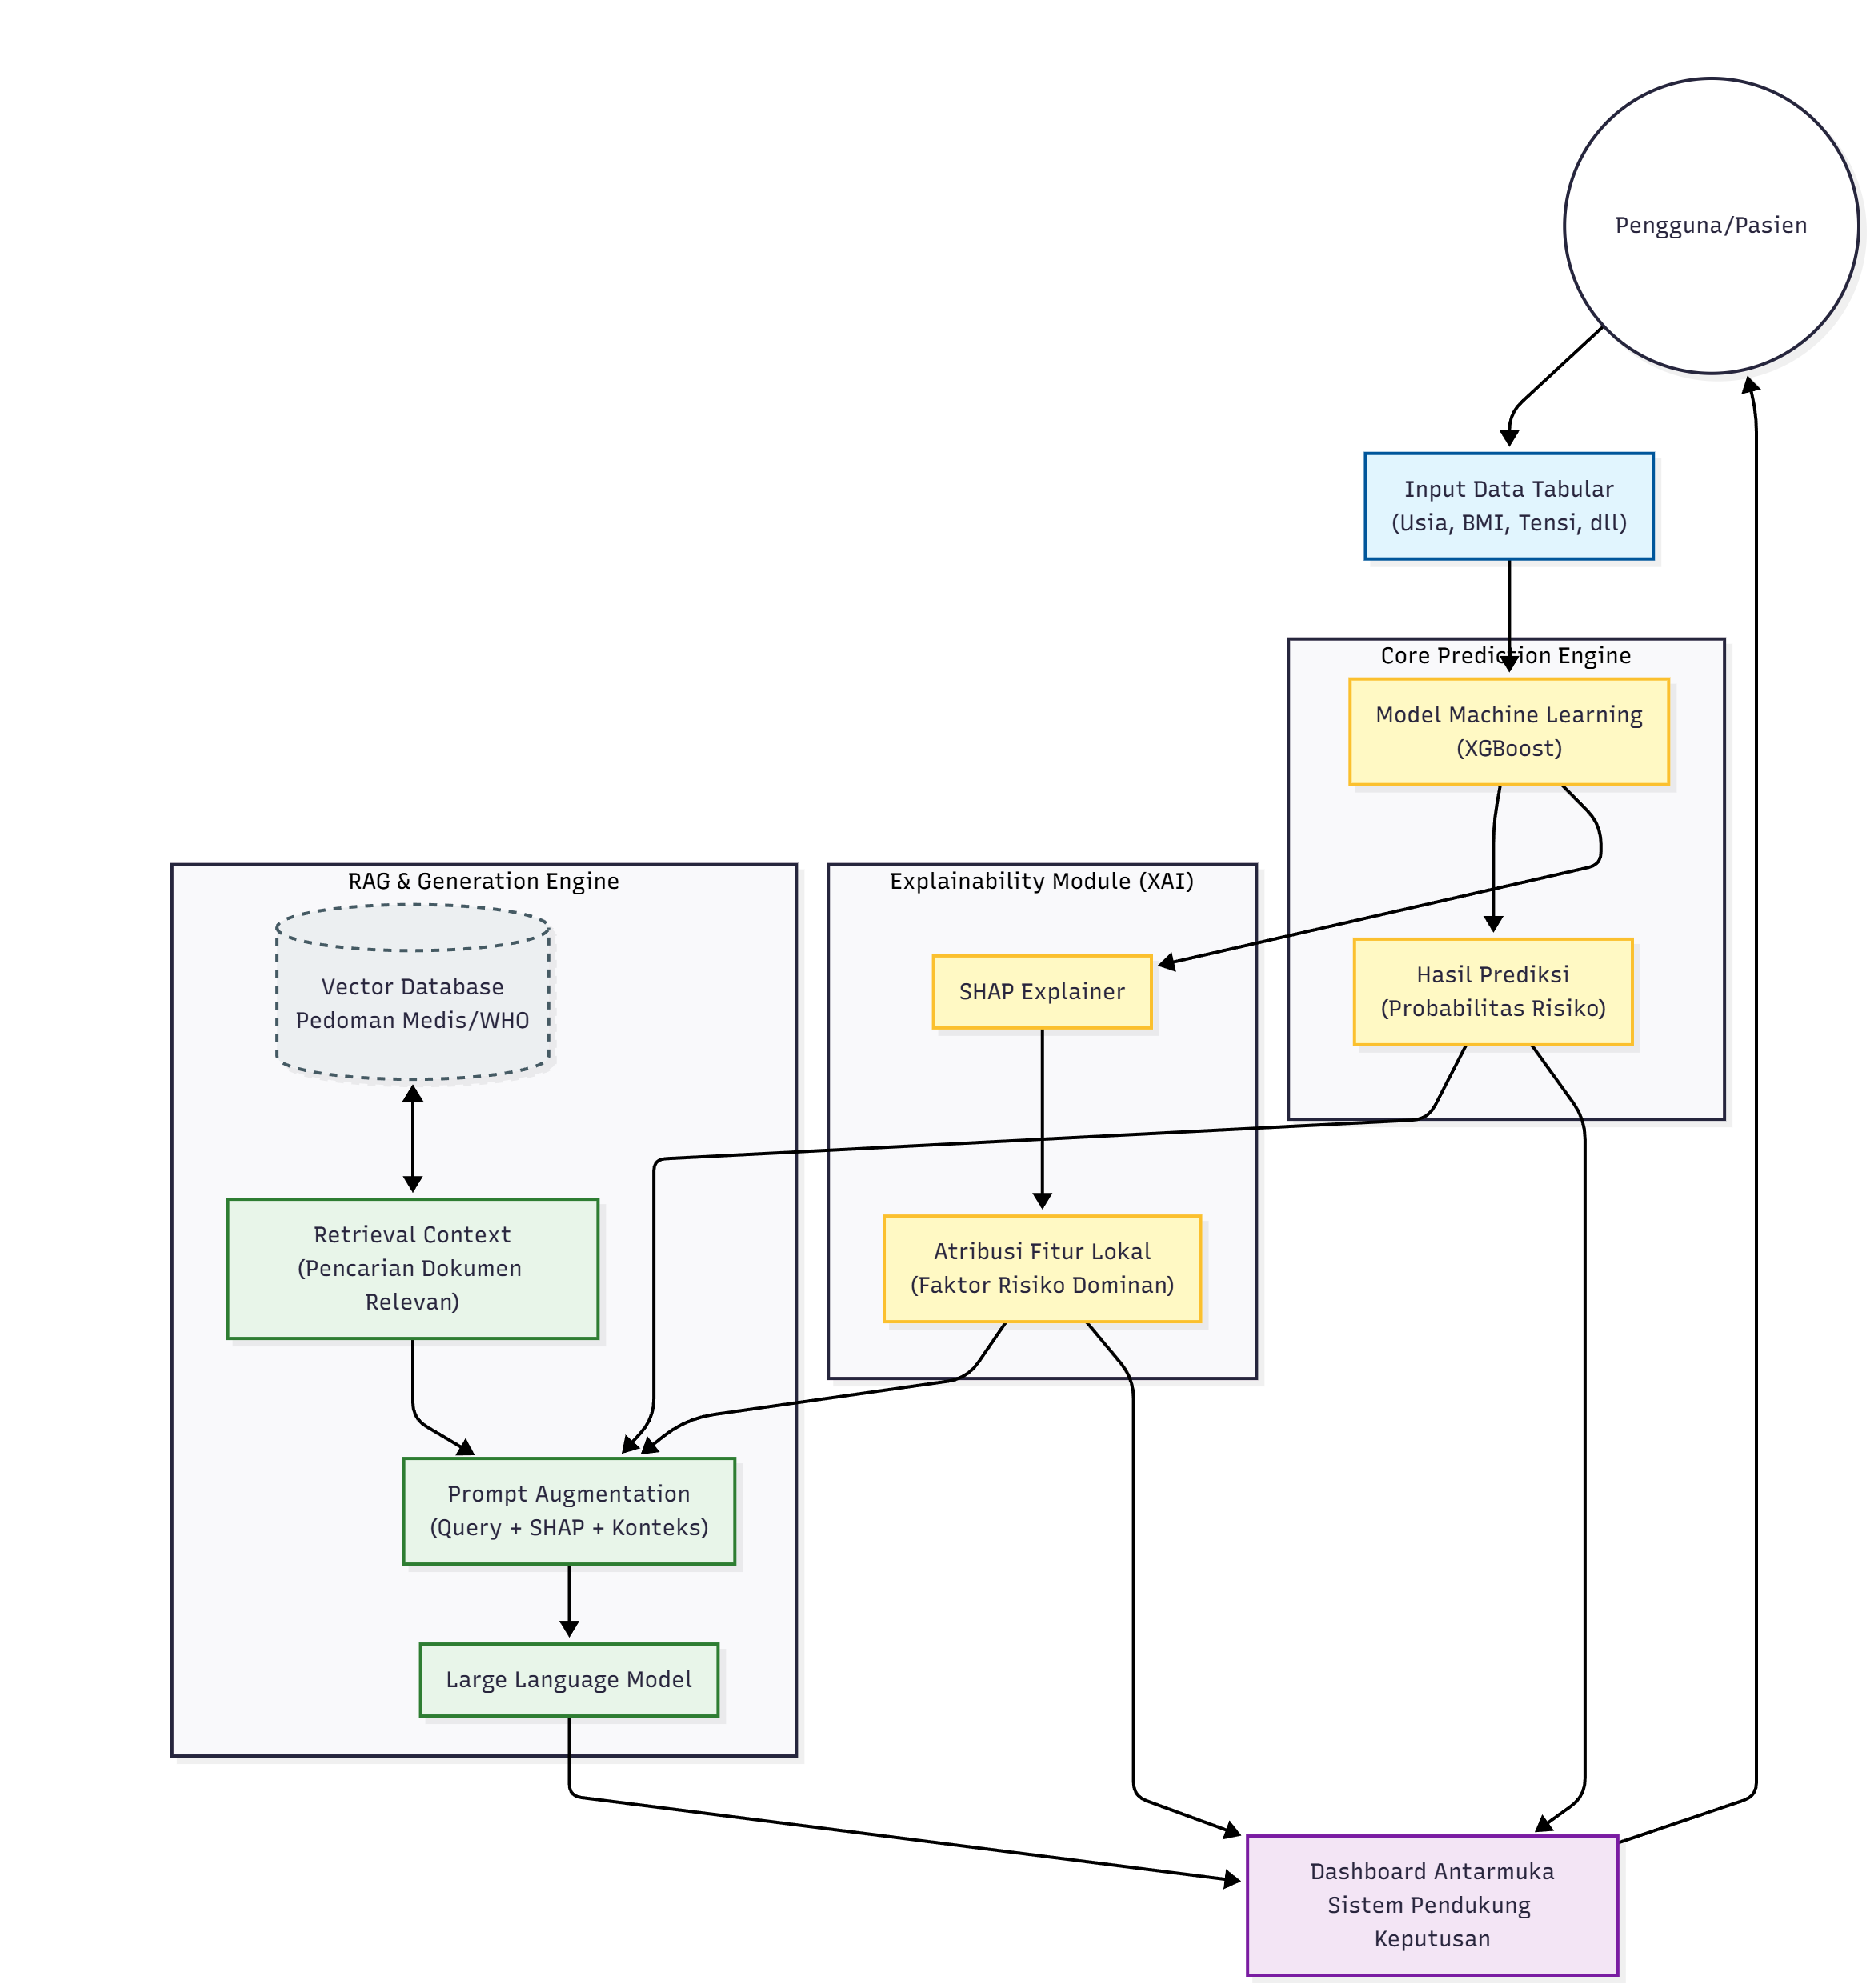
\includegraphics[width=0.8\textwidth]{image/Desain Konsep Solusi Sistem.png} 
    \caption{Desain Konsep Solusi Sistem}
    \label{fig:konsep-solusi}
\end{figure}

\subsection{Penjelasan Alur Kerja Sistem}
Sistem yang diusulkan bekerja dalam alur sekuensial otomatis sebagai berikut:

\begin{enumerate}
    \item Pengguna memasukkan parameter kesehatan (seperti usia, tekanan darah, IMT, dan riwayat keluarga) ke dalam sistem.
    
    \item Model ML (XGBoost) memproses data tersebut untuk menghasilkan skor probabilitas risiko hipertensi (misalnya: 56\% Berisiko).
    
    \item Secara paralel, modul XAI menggunakan metode SHAP untuk membedah \textit{black box} model ML. Modul ini mengidentifikasi variabel mana yang paling berkontribusi terhadap skor risiko tersebut, misalnya tinggi konsumsi garam dan IMT, yang menjadi kontributor utama.
    
    \item Sistem mengambil hasil atribusi fitur dari SHAP. Lalu setelahnya, sistem melakukan pencarian (\textit{retrieval}) pada basis data vektor yang berisi pedoman medis yang relevan dengan faktor risiko yang ditemukan, seperti pedoman dari Kemenkes atau WHO. LLM akan menggabungkan hasil prediksi, alasan dari SHAP, dan referensi medis untuk menyusun narasi penjelasan yang personal dan valid.
    
    \item Pengguna menerima tiga luaran terintegrasi: Status Risiko (ML), Grafik Faktor Penyebab (XAI), dan Penjelasan Naratif serta Saran Medis (RAG-LLM).
\end{enumerate}

\subsection{Arsitektur Sistem}
Setelah merancang alur kerja operasional sistem yang baru, langkah krusial berikutnya adalah menerjemahkan kebutuhan fungsional tersebut ke dalam spesifikasi teknis yang konkret. Diagram arsitektur sistem diperlukan untuk memetakan bagaimana komponen perangkat lunak, aliran data, dan infrastruktur saling berinteraksi guna menjalankan logika prediksi secara stabil, aman, dan skalabel.

Gambar \ref{fig:arsitektur-teknis} berikut mengilustrasikan arsitektur teknis sistem yang dirancang dengan pendekatan berbasis layanan (\textit{service-based architecture}).

\begin{figure}[h]
    \centering
    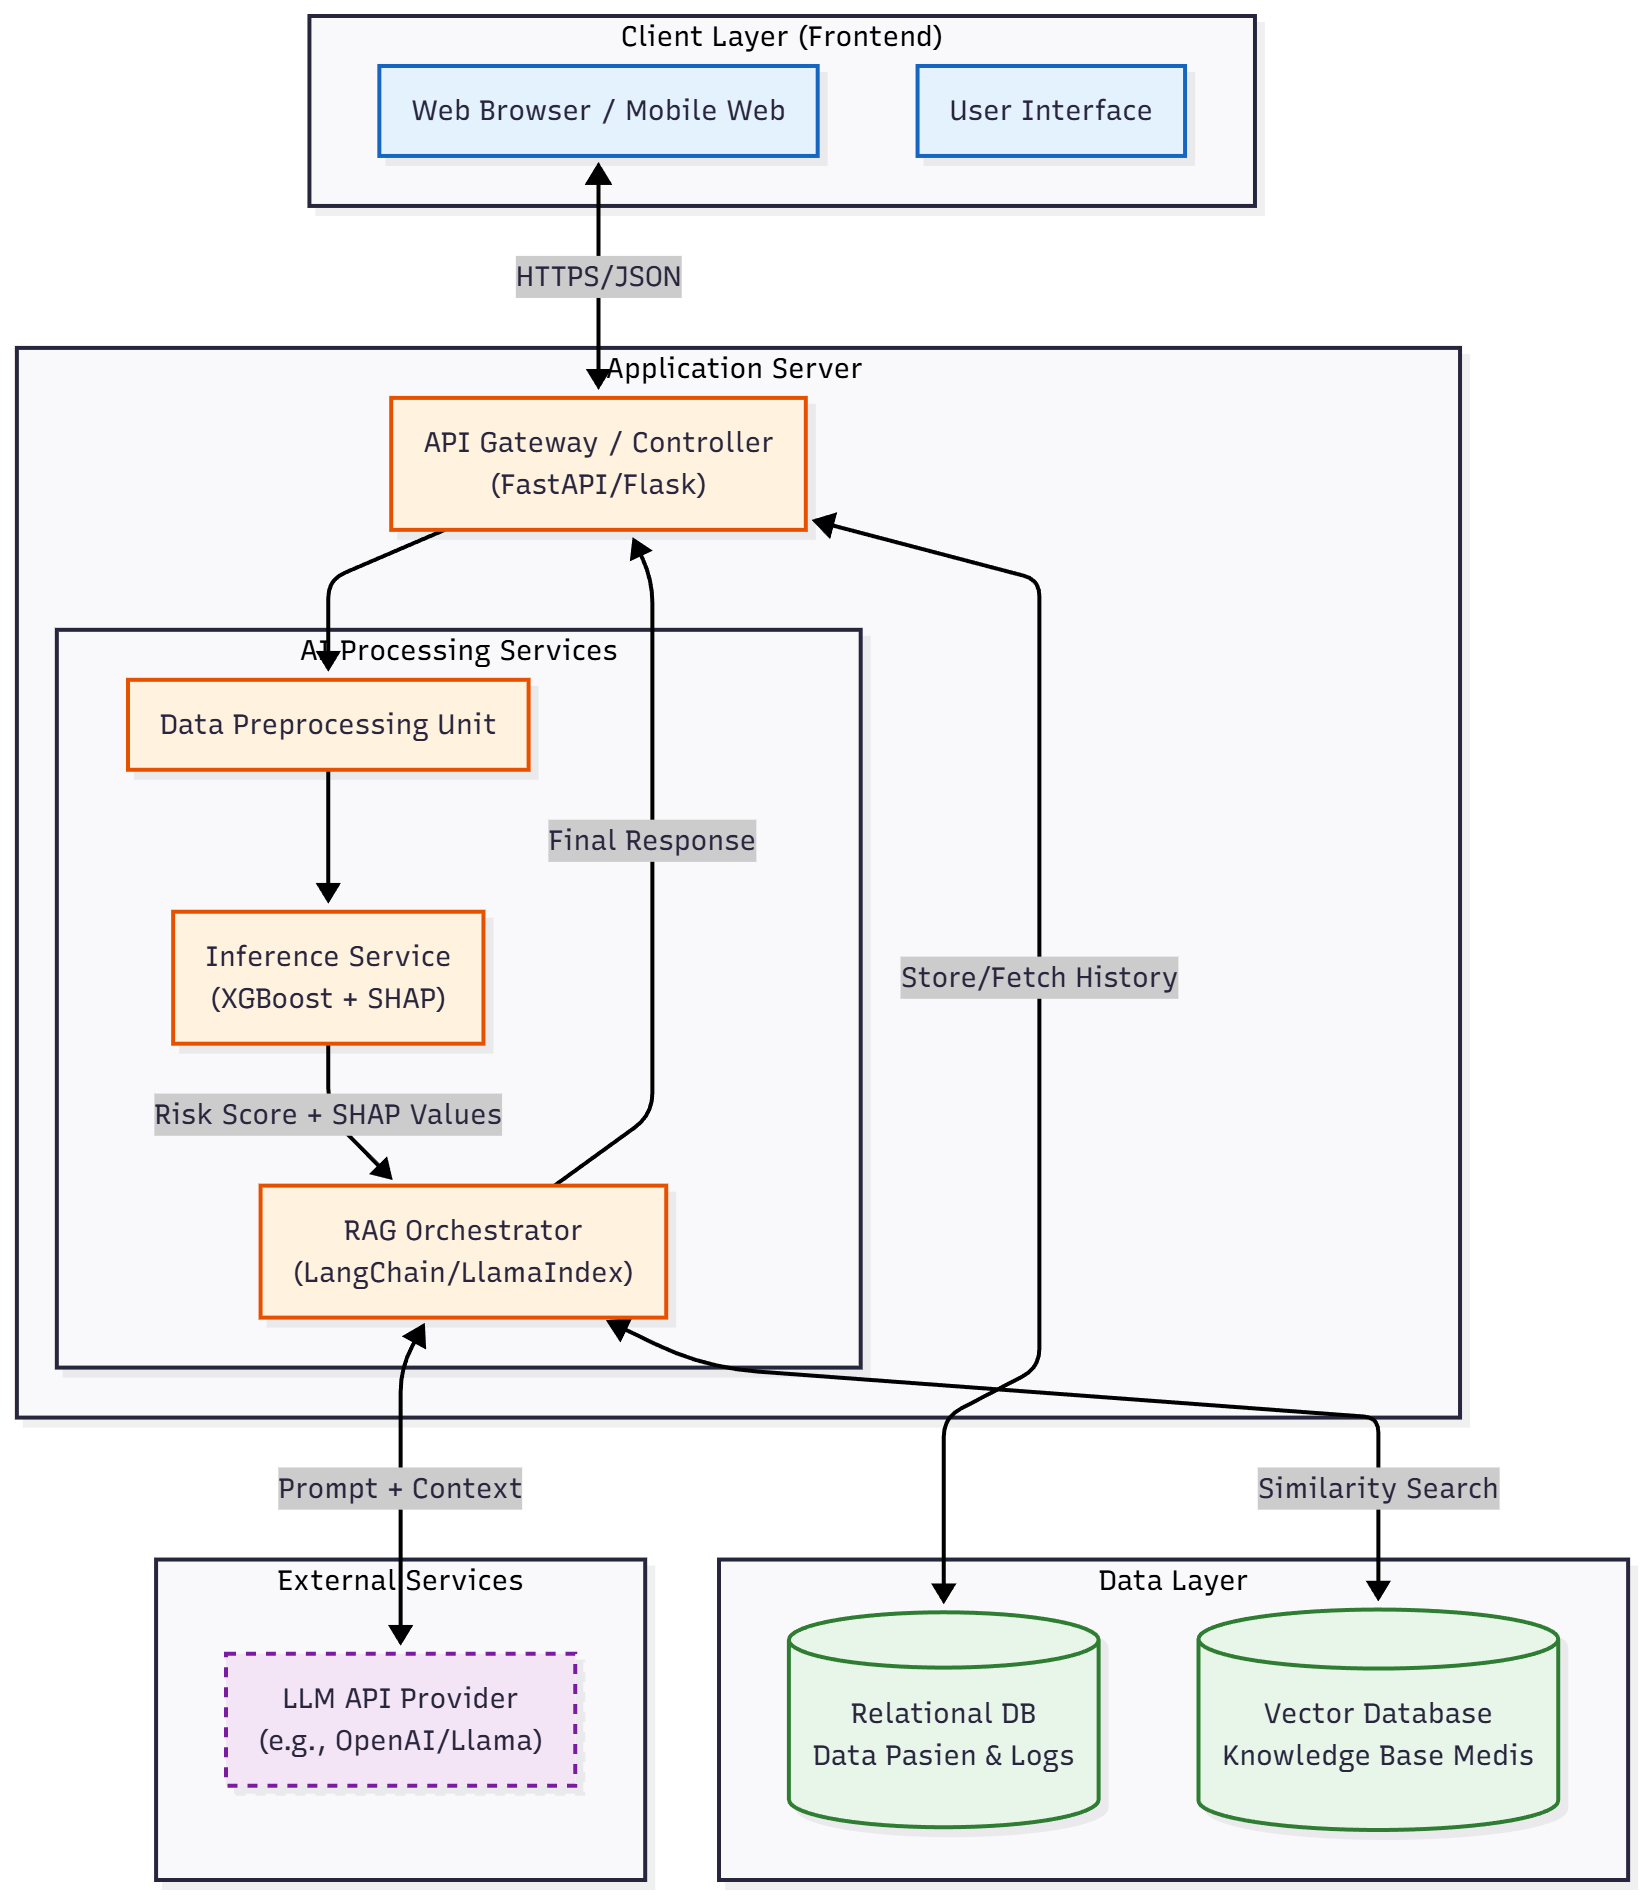
\includegraphics[width=0.8\textwidth]{image/arsitektur sistem.png}
    \caption{Arsitektur Teknis Sistem }
    \label{fig:arsitektur-teknis}
\end{figure}

Berdasarkan Gambar \ref{fig:arsitektur-teknis} di atas, sistem terbagi menjadi empat lapisan utama dengan fungsi spesifik sebagai berikut:

\begin{itemize}
    \item Client Layer (Frontend) \\
    Lapisan ini merupakan titik interaksi pengguna, baik melalui peramban web desktop maupun perangkat seluler. Lapisan ini bertugas menangkap input data klinis pasien dan memvisualisasikan hasil prediksi berupa grafik risiko dan narasi penjelasan yang dikirimkan oleh server melalui protokol HTTPS/JSON yang aman.

    \item Application Layer \\
    Lapisan ini berfungsi sebagai otak pemrosesan sistem. Lapisan ini terdiri dari API Gateway yang mengatur lalu lintas data, serta unit AI Processing Services yang menjalankan tiga fungsi sekuensial:
    \begin{enumerate}
        \item \textit{Data Preprocessing} untuk membersihkan input.
        \item \textit{Inference Service} yang menjalankan model XGBoost dan SHAP untuk menghitung skor risiko.
        \item \textit{RAG Orchestrator} yang meramu \textit{prompt} untuk model bahasa.
    \end{enumerate}

    \item Data Layer \\
    Lapisan ini bertanggung jawab atas persistensi data dengan menggunakan dua jenis basis data. \textit{Relational Database} digunakan untuk menyimpan data terstruktur pasien dan log riwayat prediksi, sedangkan \textit{vector database} digunakan khusus untuk menyimpan \textit{embedding} dokumen pedoman medis yang memungkinkan pencarian konteks semantik (\textit{similarity search}) yang cepat.

    \item External Services \\
    Sistem terhubung dengan penyedia layanan \textit{Large Language Model} (LLM) pihak ketiga seperti OpenAI atau model \textit{open-source} terhosting lainnya. Komponen ini menerima \textit{prompt} yang telah diperkaya dengan konteks medis dari sistem internal untuk menghasilkan narasi penjelasan yang natural, namun tetap tervalidasi.
\end{itemize}

\section{Perbandingan dengan Sistem Saat Ini}
Desain konsep solusi di atas menawarkan perubahan paradigma dari pendekatan konvensional yang digambarkan pada Bab III menjadi pendekatan berbasis kecerdasan buatan yang terintegrasi. Perbandingan komparatif antara kondisi saat ini (\textit{As-Is}) dan solusi yang diusulkan (\textit{To-Be}) dirangkum dalam Gambar \ref{fig:alur-diagnosis}.

% \begin{table}[htbp]
%     \centering
%     \caption{Perbandingan Sistem Konvensional vs Sistem Usulan}
%     \label{tab:perbandingan-sistem}
%     \renewcommand{\arraystretch}{1.5} % Menambah jarak antar baris agar lebih rapi
%     \begin{tabular}{|p{3.5cm}|p{5.5cm}|p{5.5cm}|}
%     \hline
%     \textbf{Aspek Pembanding} & \textbf{Sistem Saat Ini (As-Is)} & \textbf{Solusi Usulan (To-Be)} \\
%     \hline
%     Pendekatan Diagnosis & 
%     Reaktif \& Manual. Diagnosis bergantung pada pengukuran sesaat di klinik dan ingatan dokter terhadap pedoman. & 
%     Prediktif \& Otomatis. Sistem memprediksi risiko secara dini berdasarkan pola data historis menggunakan \textit{Machine Learning}. \\
%     \hline
%     Transparansi Keputusan & 
%     Intuitif/Implisit. Keputusan dokter didasarkan pada \textit{tacit knowledge} yang sulit dijelaskan secara kuantitatif kepada pasien. & 
%     \textit{Explainable} (XAI). Sistem menyediakan visualisasi atribusi fitur (SHAP) yang menunjukkan secara persis variabel penyebab risiko secara matematis. \\
%     \hline
%     Penyampaian Informasi & 
%     Lisan \& Terbatas. Penjelasan risiko sering kali singkat karena keterbatasan waktu konsultasi, menyebabkan pasien kurang paham. & 
%     Narasi Personal (GenAI). LLM menghasilkan penjelasan tertulis yang disesuaikan dengan profil pasien, menjabarkan hubungan sebab-akibat dengan bahasa alami. \\
%     \hline
%     Validitas Referensi & 
%     Variatif. Sangat bergantung pada \textit{update} pengetahuan tenaga medis masing-masing. & 
%     Terstandarisasi (RAG). Setiap saran yang dihasilkan divalidasi silang (\textit{cross-reference}) dengan dokumen pedoman medis terkini di \textit{Vector Database}. \\
%     \hline
%     Alur Kerja & 
%     Linear dan membutuhkan eskalasi manual bertingkat (perawat $\rightarrow$ dokter). & 
%     Terintegrasi dan \textit{real-time}, memberikan \textit{second opinion} instan sebelum eskalasi ke ahli. \\
%     \hline
%     \end{tabular}
% \end{table}

\begin{figure}[H]
    \centering
    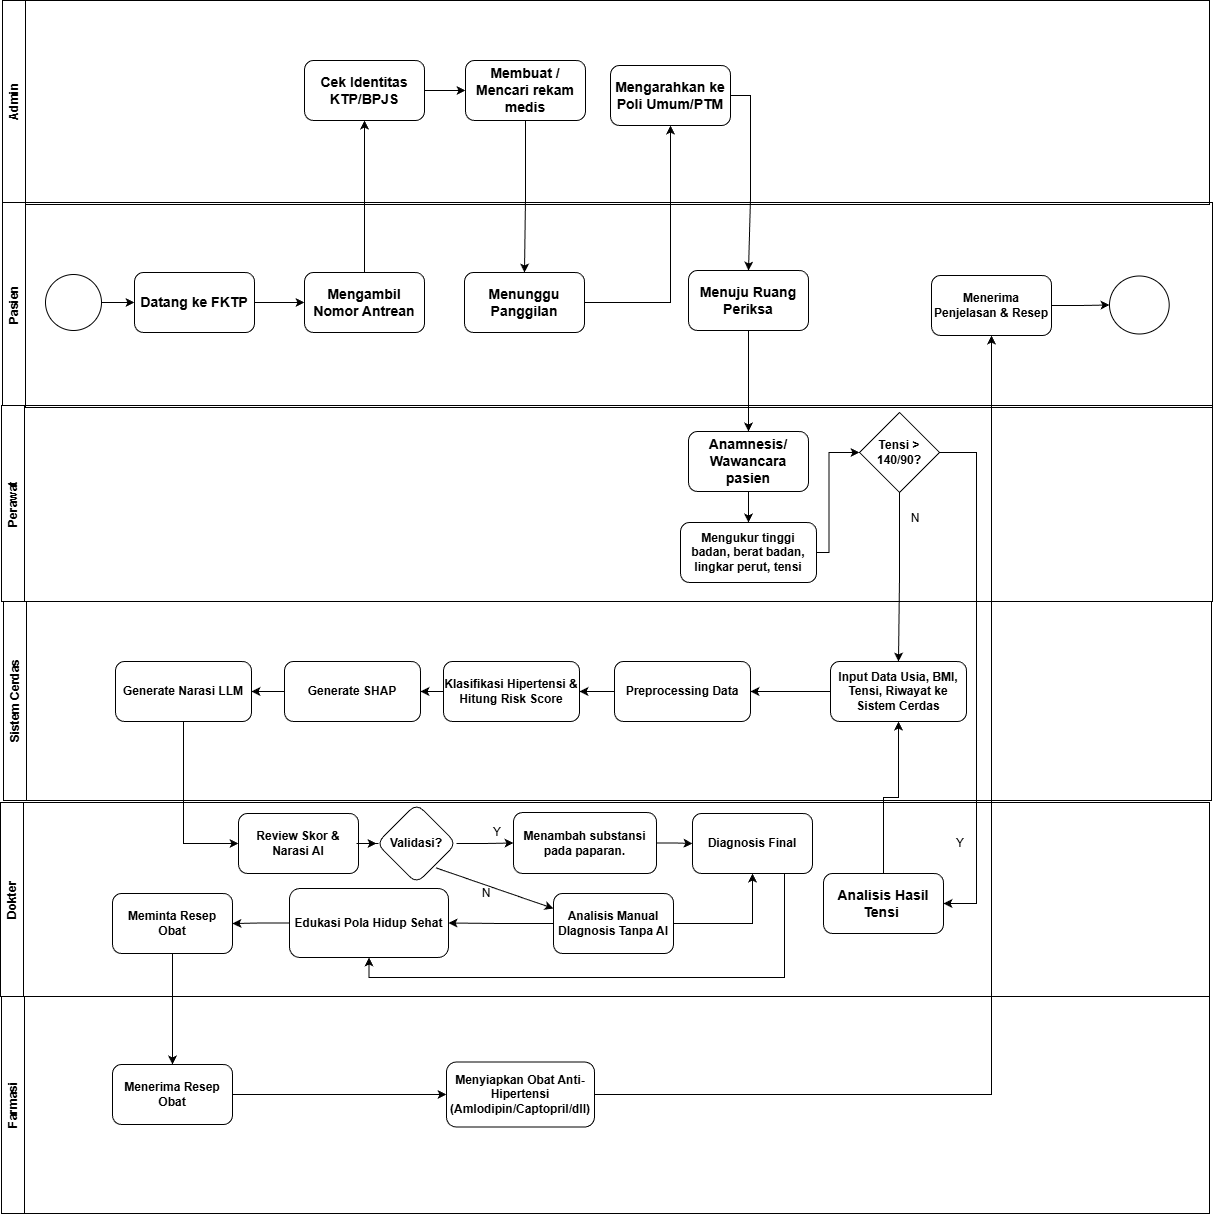
\includegraphics[width=0.8\textwidth]{image/alursistemtobe.png}
    \caption{Alur Diagnosis Hipertensi di Fasilitas Kesehatan Tingkat Pertama (FKTP) (To-Be)}
    \label{fig:alur-diagnosis}
\end{figure}

Secara visual, jika dibandingkan dengan kondisi awal, desain usulan menggambarkan adanya otomatisasi dalam proses penalaran klinis. Pada tahap ini, dokter tidak lagi melakukan observasi data pasien secara manual, melainkan memasukkan data tersebut ke dalam sistem yang berfungsi sebagai pendukung dalam pengambilan keputusan.

Meskipun demikian, penekanan utama tetap berada pada peran dokter sebagai pengambil keputusan akhir. Informasi maupun rekomendasi yang diberikan sistem harus dipahami, ditafsirkan, dan dievaluasi kembali oleh dokter untuk memperoleh wawasan klinis yang komprehensif. Dengan demikian, sistem ini dirancang bukan untuk menggantikan fungsi dokter dalam menentukan keputusan medis, tetapi untuk mengurangi beban kognitif dalam proses analisis data sehingga dokter dapat membuat keputusan yang lebih tepat, efisien, dan berbasis informasi. % Uncomment jika file sudah ada
% % ==========================================
% BAB V RENCANA SELANJUTNYA
% ==========================================
\chapter{RENCANA SELANJUTNYA}
\label{chap:rencana-selanjutnya}


\section{Implementasi}
Bagian ini meliputi kakas dan lingkungan implementasi, implementasi dataset, \textit{machine learning}, XAI, dan implementasi model ke aplikasi.

\subsection{Kakas dan Lingkungan Implementasi}
Implementasi dilakukan dengan memanfaatkan berbagai perangkat lunak pendukung yang berperan dalam pemrosesan data, pengembangan model \textit{Machine Learning}, integrasi XAI, serta penyusunan narasi klinis dengan pendekatan \textit{Retrieval Augmented Generation}. Kakas yang digunakan dapat diklasifikasikan ke dalam beberapa kelompok berikut:

\begin{enumerate}
    \item \textbf{Python}: Digunakan sebagai bahasa pemrograman utama dalam seluruh tahapan pengembangan model yang meliputi pemrosesan data, pelatihan model prediksi, integrasi XAI, serta komponen \textit{backend} pada prototipe aplikasi.
    \item \textbf{NumPy}: Digunakan untuk operasi komputasi numerik dan manipulasi struktur \textit{array}.
    \item \textbf{Pandas}: Digunakan untuk eksplorasi data tabular, pembersihan data, transformasi variabel, serta penyusunan dataset pelatihan dan pengujian.
    \item \textbf{Matplotlib dan Seaborn}: Digunakan untuk menampilkan grafik terkait distribusi variabel, korelasi fitur klinis, dan visualisasi metrik evaluasi model.
    \item \textbf{Scikit-learn}: Digunakan untuk \textit{preprocessing} data, pembagian dataset, penghitungan metrik evaluasi, serta \textit{baseline model}.
    \item \textbf{XGBoost}: Digunakan sebagai algoritma utama klasifikasi risiko hipertensi yang sebelumnya telah dipilih berdasarkan evaluasi performa pada dataset tabular dengan variabel risiko multidimensional.
    \item \textbf{SHAP}: Diterapkan untuk memberikan interpretasi luaran model baik dalam skala lokal maupun global. Metode ini mampu mengukur kontribusi setiap fitur secara matematis dengan prinsip keadilan dan konsistensi. Oleh karena itu, instrumen ini menjadi krusial dalam mengevaluasi keandalan model serta menjamin transparansi, khususnya pada sistem estimasi risiko medis yang sensitif seperti hipertensi.
    \item \textbf{LangChain}: Digunakan sebagai kerangka integrasi untuk pipeline \textit{Retrieval Augmented Generation} meliputi komponen \textit{retriever}, pemanggilan model, pemrosesan konteks, dan orkestrasi \textit{prompt}.
    \item \textbf{OpenAI API}: Digunakan untuk menghasilkan narasi klinis berbasis konteks serta mendukung proses evaluasi faktualitas melalui \textit{prompt engineering}.
\end{enumerate}

Lingkungan implementasi yang digunakan dalam penelitian ini meliputi perangkat keras dan perangkat lunak berikut:

\begin{enumerate}
    \item \textbf{Perangkat Keras}
    \begin{enumerate}
        \item Laptop: Lenovo IdeaPad Gaming 3 15ACH6
        \item Processor (CPU): AMD Ryzen 5 5600H with Radeon Graphics
        \item Memori (RAM): 16 GB
        \item Penyimpanan: SSD 954 GB
    \end{enumerate}
    \item \textbf{Perangkat Lunak}
    \begin{enumerate}
        \item Sistem operasi: Windows 11
        \item Editor dan IDE: Visual Studio Code dan Jupyter Notebook
    \end{enumerate}
\end{enumerate}

\subsection{Jadwal Implementasi}
Jadwal pelaksanaan penelitian dirinci dalam bentuk tabel kegiatan. Estimasi waktu relatif untuk setiap tahapan pekerjaan adalah sebagai berikut. Berikut adalah penjelasan detail dari jadwal penelitian dan pengembangan proyek. Tabel ini merinci setiap tahapan penelitian dan proyek, aktivitas utama, dan durasinya, sesuai dengan jadwal yang telah direncanakan.

\begin{table}[H]
    \caption{Tabel Detail Jadwal Proyek}
    \label{tab:jadwal-proyek}
    \centering
    \small
    \begin{tabular}{|p{1.5cm}|p{4.5cm}|p{3cm}|p{2cm}|p{2cm}|}
        \hline
        \textbf{Kode} & \textbf{Kegiatan} & \textbf{Output} & \textbf{Durasi} & \textbf{PIC} \\
        \hline
        BU-01 & Finalisasi ruang lingkup \& kebutuhan pengguna & Dokumen kebutuhan & 2 bulan & Peneliti \\
        \hline
        BU-02 & Studi literatur lanjutan AI/XAI/RAG medis & Bab II lengkap & 2 bulan & Peneliti \\
        \hline
        DU-01 & Akuisisi \& \textit{pre-assessment} dataset & Dataset siap analisis & 3 bulan & Peneliti \\
        \hline
        DP-01 & Data cleaning \& \textit{preprocessing} & Dataset siap model & 3 bulan & Peneliti \\
        \hline
        DP-02 & Feature engineering + balancing & Dataset final model & 3 bulan & Peneliti \\
        \hline
        ML-01 & Model training XGBoost + \textit{fine-tuning} & Model 70\% akurasi (target) & 2 bulan & Peneliti \\
        \hline
        XAI-01 & SHAP attribution analysis & Visualisasi kontribusi fitur & 2 bulan & Peneliti \\
        \hline
        RAG-01 & VectorDB + indexing pedoman medis & Knowledge base terstruktur & 2 bulan & Peneliti \\
        \hline
        RAG-02 & Integrasi LLM + narasi klinis & Penjelasan dapat dimengerti & 2 bulan & Peneliti \\
        \hline
        EV-01 & Evaluasi ML (Accuracy, Precision, F1) & Laporan performa model & 2 bulan & Peneliti \\
        \hline
        EV-02 & Evaluasi RAG (RAGAS: Faithfulness dll.) & Laporan evaluasi narasi & 2 bulan & Peneliti \\
        \hline
        DEP-01 & Pengembangan web prototype & Sistem CDSS berbasis web & 3 bulan & Peneliti \\
        \hline
        DEP-02 & User testing (dokter/tenaga medis) & Feedback usability \& klinis & 2 bulan & Peneliti \\
        \hline
        DOC-01 & Penyusunan laporan TA \& publikasi & Draft TA lengkap & 10 bulan & Peneliti \\
        \hline
    \end{tabular}
\end{table}


\section{Desain pengujian dan evaluasi}
Evaluasi dilakukan untuk menilai kinerja model serta meninjau rasionalitas keputusan yang dihasilkan dengan melibatkan ahli di bidangnya. Tujuan dari proses ini adalah memastikan bahwa model tidak hanya mampu memprediksi risiko hipertensi secara akurat, tetapi juga menghasilkan penalaran yang logis, mudah dipahami, dan dapat dipertanggungjawabkan dalam praktik medis.

\subsection{Evaluasi Kinerja Model}
Pengujian kinerja model direncanakan menggunakan himpunan data uji terpisah untuk memvalidasi kemampuan generalisasi model dalam mengklasifikasikan risiko hipertensi. Sesuai dengan batasan masalah yang telah ditetapkan, evaluasi kuantitatif akan berfokus pada metrik \textit{Receiver Operating Characteristic Area Under Curve} atau ROC-AUC dan \textit{Precision-Recall Area Under Curve} atau PR-AUC sebagai indikator utama keberhasilan.

Penggunaan ROC-AUC dipilih karena metrik ini mampu mengukur kinerja pemisahan kelas oleh model di berbagai ambang batas klasifikasi secara komprehensif. Mengingat luaran model berupa probabilitas risiko dan bukan sekadar label biner, ROC-AUC menjadi instrumen vital untuk melihat seberapa konsisten model memberikan skor risiko yang lebih tinggi pada pasien hipertensi dibandingkan pasien sehat.

Selain itu, rencana evaluasi akan memberikan bobot prioritas pada nilai \textit{Sensitivity} atau \textit{Recall}. Hal ini didasarkan pada karakteristik hipertensi sebagai \textit{the silent killer} yang sering tidak bergejala. Dalam konteks penapis kesehatan, kegagalan mendeteksi pasien berisiko atau \textit{False Negative} memiliki konsekuensi keselamatan yang jauh lebih fatal dibandingkan kesalahan deteksi pada orang sehat. Oleh karena itu, skenario pengujian akan dirancang untuk memastikan model mencapai target \textit{Recall} yang optimal, sebagaimana ditargetkan dalam kebutuhan nonfungsional sistem.

Metrik pendukung seperti \textit{Specificity} dan F1-Score juga akan dilibatkan untuk memantau keseimbangan model, terutama dalam menghadapi potensi ketidakseimbangan kelas pada dataset. \textit{Specificity} diperlukan untuk menjaga kepercayaan pengguna dengan tidak terlalu sering memberikan peringatan palsu, sedangkan F1-Score akan menjadi acuan harmonisasi antara ketepatan dan daya cakup prediksi. Kinerja model nantinya akan dibandingkan dengan ambang batas dasar atau \textit{baseline} dari penelitian terdahulu untuk memastikan bahwa solusi yang diusulkan memiliki nilai kompetitif secara ilmiah.

\subsection{Rencana Evaluasi Rasionalitas Model}
Evaluasi rasionalitas dirancang untuk memverifikasi validitas logika medis yang dipelajari oleh algoritma \textit{Machine Learning}. Tahapan ini tidak hanya melihat hasil akhir prediksi, tetapi menelusuri alur pengambilan keputusan menggunakan metode \textit{Explainable Artificial Intelligence} atau XAI, khususnya \textit{Shapley Additive exPlanations} atau SHAP.

Mekanisme validasi akan dilaksanakan melalui konsultasi dengan tenaga ahli medis atau dokter. Dalam proses ini, sejumlah sampel kasus uji akan disajikan bersamaan dengan visualisasi nilai SHAP yang menunjukkan fitur-fitur dominan yang memengaruhi skor risiko. Tenaga ahli kemudian akan diminta menilai kesesuaian antara fitur yang dianggap penting oleh model dengan pedoman klinis standar, seperti panduan dari Kementerian Kesehatan atau organisasi hipertensi internasional.

Sebagai indikator keberhasilan evaluasi ini, model diharapkan mampu menunjukkan pola kausalitas yang benar. Misalnya, peningkatan variabel usia, indeks massa tubuh, atau riwayat tekanan darah sistolik harus berkontribusi positif terhadap kenaikan skor risiko hipertensi. Sebaliknya, model harus dapat mengenali faktor protektif atau variabel yang menurunkan risiko. Jika interpretasi model dinilai selaras dengan pengetahuan medis dan bebas dari korelasi semu yang menyesatkan, maka model akan dinyatakan lolos uji rasionalitas dan layak diintegrasikan dengan komponen \textit{Large Language Model} untuk tahap pembangkitan narasi.

\subsection{Evaluasi RAG}
Sistem yang diusulkan mengevaluasi kinerja arsitektur \textit{Retrieval-Augmented Generation} (RAG) menggunakan kerangka kerja evaluasi standar yaitu \textit{Retrieval Augmented Generation Assessment} (RAGAS). Pendekatan ini dipilih karena metrik tradisional dianggap tidak memadai untuk mengukur koherensi semantik dan akurasi faktual yang dihasilkan oleh \textit{Large Language Model} (LLM) dalam konteks RAG. RAGAS beroperasi secara \textit{reference-free} dengan memanfaatkan LLM itu sendiri sebagai juri penilai, yang terbukti memiliki korelasi tinggi dengan penilaian manusia. Evaluasi ini memisahkan proses penilaian menjadi dua komponen utama, yaitu metrik kualitas generasi teks (\textit{generation}) dan metrik kualitas pengambilan konteks (\textit{retrieval}).

Berikut adalah penjelasan mengenai metrik-metrik kunci dalam evaluasi RAGAS yang diterapkan:

\begin{enumerate}
    \item \textbf{Faithfulness}\\ Kerangka RAGAS mengukur \textit{Faithfulness} untuk menilai konsistensi faktual dari narasi yang dibangkitkan terhadap konteks yang disajikan oleh \textit{retriever}. Metrik ini menjadi sangat krusial dalam domain kesehatan yang berisiko tinggi karena berfungsi untuk memastikan bahwa model tidak menghasilkan informasi medis yang dibuat-buat atau halusinasi. Hal ini secara langsung memitigasi bahaya laten yang timbul dari fabrikasi saran medis dan melanggar prinsip etika medis (\textit{non-maleficence}). Dengan demikian, \textit{Faithfulness} menjamin bahwa respons model memiliki landasan bukti (\textit{evidence-grounded}) yang dapat diverifikasi demi keselamatan pasien.
    
    \item \textbf{Context Precision}\\ Digunakan untuk mengevaluasi kualitas pengambilan dokumen. Metrik ini menghitung rasio antara informasi yang relevan yang berhasil diambil dibandingkan dengan total informasi yang disajikan. Nilai presisi konteks yang tinggi menunjukkan efisiensi sistem dalam menyaring data medis yang tidak diperlukan atau \textit{noise data}. Pengukuran ini sangat penting karena ketidaksinkronan antara proses \textit{retrieval} dan \textit{generation} dapat terjadi jika informasi yang tidak relevan masuk ke dalam konteks, yang pada akhirnya dapat memengaruhi kualitas penjelasan akhir.
    
    \item \textbf{Context Recall}\\ Mengukur kemampuan sistem untuk mengambil seluruh informasi yang diperlukan dari basis pengetahuan eksternal guna menjawab pertanyaan pengguna secara komprehensif. Kualitas metrik ini sangat memengaruhi \textit{prompt} yang diperkaya (\textit{augmented}) yang diberikan kepada LLM, memastikan model memiliki fondasi faktual yang lengkap sebelum menyusun jawaban. Dalam konteks medis, metrik ini juga didukung oleh \textit{Context Entity Recall} yang memastikan entitas spesifik krusial (seperti nama obat atau kondisi komorbiditas hipertensi) tidak hilang selama pengambilan konteks.
    
    \item \textbf{Answer Relevancy}\\ Metrik ini menilai kualitas narasi yang dibangkitkan dari perspektif sejauh mana jawaban tersebut secara langsung merespons pertanyaan yang diajukan oleh pengguna. Metrik \textit{Answer Relevancy} diukur tanpa mempertimbangkan kebenaran faktual dari jawaban yang dihasilkan. Tujuannya adalah untuk memastikan bahwa LLM tetap fokus pada permintaan pengguna, yang krusial dalam menghasilkan output yang mudah dipahami dan personal bagi pasien maupun tenaga medis.
\end{enumerate}

\section{Analisis Risiko dan Mitigasi}
Sistem yang diusulkan beroperasi dalam ranah kesehatan yang menuntut akurasi faktual dan keandalan keputusan sehingga manajemen risiko harus diterapkan secara sistematis. Analisis ini mengadopsi prinsip dan proses dari pedoman Manajemen Risiko ISO 31000 yang membagi prosesnya menjadi tiga tahapan besar yaitu identifikasi risiko, analisis dan evaluasi risiko, serta penanganan risiko.

\subsection{Identifikasi Risiko Kunci}
Identifikasi risiko berfokus pada potensi kegagalan di setiap komponen sistem hibrida yang dapat memengaruhi keselamatan pasien dan kepercayaan klinis. Komponen tersebut meliputi \textit{Machine Learning} (ML), \textit{Explainable Artificial Intelligence} (XAI), dan \textit{Retrieval Augmented Generation} (RAG). Risiko-risiko kunci yang teridentifikasi adalah sebagai berikut:

\begin{enumerate}
    \item \textbf{Risiko Halusinasi Medis (R1)}\\ 
    Model bahasa besar atau LLM rentan menghasilkan informasi yang difabrikasi yaitu informasi yang terdengar meyakinkan namun faktanya salah. Dampak potensial dari risiko ini adalah bahaya keselamatan pasien yang fatal jika sistem memberikan saran medis yang tidak berdasar atau bertentangan dengan pedoman klinis resmi.
    \item \textbf{Risiko Kegagalan Faithfulness (R2)} \\ 
    Jawaban yang dihasilkan oleh LLM tidak sepenuhnya didukung oleh konteks yang diambil dari basis data vektor atau \textit{Vector Database}. Hal ini menunjukkan ketidaksetiaan faktual terhadap sumber. Dampak potensialnya adalah kerusakan kredibilitas sistem dan defisit kepercayaan di kalangan tenaga medis.
    \item \textbf{Risiko Kualitas Retrieval (R3)} \\ 
    Komponen \textit{retriever} gagal mengambil semua konteks yang relevan atau justru mengambil terlalu banyak informasi tidak relevan sehingga menyebabkan ketidaksinkronan antara proses pencarian dan pembangkitan jawaban.
    \item \textbf{Risiko Kegagalan Target Recall Model Prediksi (R4)} \\ 
    Model ML gagal mencapai target metrik sensitivitas klinis atau \textit{Recall} melampaui 70\% pada data uji. Dampak potensialnya adalah tingginya angka negatif palsu atau \textit{False Negative} yaitu pasien berisiko tinggi yang tidak terdeteksi.
    \item \textbf{Risiko Latensi Sistem Tinggi (R5)} \\ 
    Waktu tunggu total dari input data hingga munculnya narasi penjelasan melampaui batas yang ditentukan yaitu 10 detik. Hal ini mencakup proses RAG secara keseluruhan. Latensi tinggi dapat menurunkan pengalaman pengguna.
\end{enumerate}

\subsection{Analisis dan Evaluasi Risiko}
Analisis risiko dilakukan dengan membandingkan kemungkinan dan dampak setiap risiko. Mengingat sensitivitas sistem ini dalam domain kesehatan maka beberapa risiko dapat memiliki dampak yang tinggi. Oleh karena itu strategi mitigasi difokuskan pada penanganan proaktif terhadap risiko berkategori tinggi tersebut.

\subsection{Strategi Mitigasi dan Tindak Lanjut}
Strategi penanganan risiko berfokus pada mitigasi untuk mengurangi kemungkinan atau dampak dan didukung dengan rencana kontingensi sebagai tindak lanjut jika evaluasi menunjukkan kegagalan. Rincian strategi mitigasi dapat dilihat pada Tabel \ref{tab:mitigasi-risiko}.

\begin{table}[htbp]
    \caption{Strategi mitigasi risiko dan rencana tindak lanjut}
    \label{tab:mitigasi-risiko}
    \centering
    \small
    \begin{tabular}{|p{2cm}|p{5.5cm}|p{5.5cm}|}
        \hline
        \textbf{Kode Risiko} & \textbf{Strategi Mitigasi} & \textbf{Tindak Lanjut Jika Gagal} \\
        \hline
        R1 \& R2 & Menggunakan arsitektur RAG untuk secara eksplisit memaksa LLM membatasi respons pada dokumen pedoman klinis Kemenkes atau WHO. Kualitas narasi divalidasi menggunakan metrik \textit{Faithfulness} dari kerangka RAGAS. & Jika skor \textit{Faithfulness} atau \textit{Answer Relevancy} rendah maka lakukan \textit{fine-tuning} atau rekayasa \textit{prompt} ulang pada komponen generator untuk menekankan pembatasan konteks. \\
        \hline
        R3 & Evaluasi komponen \textit{retriever} menggunakan metrik \textit{Context Precision} untuk menolak data bising dan \textit{Context Recall} untuk memastikan kelengkapan dari kerangka RAGAS. & Jika skor \textit{retrieval} rendah maka lakukan \textit{fine-tuning} pada model \textit{embedding} yang digunakan untuk pencarian vektor atau terapkan mekanisme \textit{reranking} pascapencarian dokumen. \\
        \hline
        R4 & ML dioptimalkan untuk memprioritaskan metrik \textit{Recall} selama pelatihan dengan target minimal 70\% untuk meminimalkan \textit{False Negative}. & Jika \textit{Recall} kurang dari 70\% maka terapkan teknik \textit{hyperparameter tuning} yang lebih agresif pada model XGBoost atau gunakan teknik penyeimbangan data seperti SMOTE untuk mengatasi ketidakseimbangan kelas pada data latih. \\
        \hline
        R5 & Menerapkan mekanisme \textit{Semantic Cache} dan klasifikasi kueri untuk pertanyaan sederhana agar dapat melewati alur RAG penuh yang mahal secara komputasi. & Jika waktu tunggu total melampaui 10 detik maka lakukan optimasi pada proses pencarian vektor seperti penyesuaian algoritma ANNS atau pertimbangkan untuk menggunakan API LLM yang memiliki latensi lebih rendah. \\
        \hline
    \end{tabular}
\end{table} % Uncomment jika file sudah ada

\backmatter

% ==========================================
% DAFTAR PUSTAKA
% ==========================================
\printbibliography[title={DAFTAR PUSTAKA}]

% ==========================================
% LAMPIRAN (optional)
% ==========================================
\appendix
% \input{Lampiran-A.tex}

\end{document}